\documentclass[12pt, a4paper]{report}
\usepackage[utf8]{inputenc}
\usepackage{graphicx}
\graphicspath{{../images/}}
\usepackage{amsmath,amssymb,amsfonts}
\usepackage{float}
\usepackage{multirow}
\usepackage{hyperref}
\usepackage{geometry}
\geometry{a4paper, margin=1in}
\usepackage{setspace}
\usepackage{booktabs}
\usepackage{tabularx}
\usepackage{xltabular}
\usepackage{tikz}
\usetikzlibrary{positioning, shapes.multipart, arrows.meta}
\onehalfspacing

\usepackage{titlesec}
\titleformat{\chapter}[display]
  {\normalfont\huge\bfseries\centering}{\chaptertitlename\ \thechapter}{20pt}{\Huge}
\titleformat{name=\chapter,numberless}[block]
  {\normalfont\huge\bfseries\centering}{}{0pt}{}

\begin{document}

% ----------------------------------------------------------------
% COVER PAGE (USTC STANDARD)
% ----------------------------------------------------------------
\begin{titlepage}
    \centering
    \vspace*{1cm}
    
    {\Large \textbf{UNIVERSITY OF SCIENCE AND TECHNOLOGY CHITTAGONG}\par}
    {\large \textbf{BACHELOR OF SCIENCE IN COMPUTER SCIENCE AND ENGINEERING}\par}
    \vspace{2cm}
    
    {\Large \textbf{PEDIATRIC VS ADULT DENGUE SEVERITY PREDICTION WITH SUBGROUP-SPECIFIC SHAP EXPLANATIONS}\par}
    \vspace{2cm}
    
    {\large \textbf{SUBMITTED BY}\par}
    \vspace{0.3cm}
    {\large \textbf{MD. AFTABUL ISLAM} \quad ID: 22070103 \par}
    {\large \textbf{MOHAMMAD MAZHARUL ALAM} \quad ID: 22070116 \par}
    
    \vspace{1.5cm}
    {\large \textbf{SUPERVISED BY}\par}
    \vspace{0.3cm}
    {\large \textbf{MOHAMMAD ARIF HASAN CHOWDHURY}\par}
    {\large Assistant Professor\par}
    {\large Department of Computer Science and Engineering\par}
    {\large University of Science and Technology Chittagong\par}
    
    \vfill
    {\large \textbf{SUBMITTED TO}\par}
    \vspace{0.3cm}
    {\large \textbf{DEPARTMENT OF COMPUTER SCIENCE AND ENGINEERING (CSE)}\par}
    {\large \textbf{FACULTY OF SCIENCE ENGINEERING AND TECHNOLOGY (FSET)}\par}
    {\large \textbf{UNIVERSITY OF SCIENCE AND TECHNOLOGY CHITTAGONG (USTC)}\par}
    \vspace{0.5cm}
    {\large July, 2026\par}
\end{titlepage}

% ----------------------------------------------------------------
% INNER TITLE PAGE
% ----------------------------------------------------------------
\begin{titlepage}
    \centering
    \vspace*{1.5cm}
    
    {\Large \textbf{Pediatric vs Adult Dengue Severity Prediction with Subgroup-Specific SHAP Explanations}\par}
    % \vspace{0.5cm}
    % {\Large \textbf{Age-Stratified Machine Learning for a Hematology-Based Dengue Severity Proxy: Leakage Control, Cross-Source Validation, and SHAP Analysis}\par}
    \vspace{1.5cm}
    
    {\large \textbf{Submitted by:}\par}
    \vspace{0.3cm}
    {\large \textbf{MD. AFTABUL ISLAM} \\ ID: 22070103 \par}
    \vspace{0.2cm}
    {\large \textbf{MOHAMMAD MAZHARUL ALAM} \\ ID: 22070116 \par}
    
    \vspace{1.5cm}
    {\large \textbf{Supervised by:}\par}
    \vspace{0.3cm}
    {\large \textbf{Mohammad Arif Hasan Chowdhury}\par}
    {\large Assistant Professor\par}
    {\large Department of Computer Science and Engineering\par}
    {\large University of Science and Technology Chittagong\par}
    
    \vfill
    {\large In partial fulfillment of the requirement for the Degree of Bachelor of Science in Computer Science and Engineering, University of Science and Technology Chittagong.\par}
    \vspace{1cm}
    {\large \textbf{DEPARTMENT OF COMPUTER SCIENCE AND ENGINEERING (CSE)}\par}
    {\large \textbf{FACULTY OF SCIENCE ENGINEERING AND TECHNOLOGY (FSET)}\par}
    {\large \textbf{UNIVERSITY OF SCIENCE AND TECHNOLOGY CHITTAGONG (USTC)}\par}
\end{titlepage}

\pagenumbering{roman}

% ----------------------------------------------------------------
% DECLARATION
% ----------------------------------------------------------------
\chapter*{DECLARATION}
\addcontentsline{toc}{chapter}{DECLARATION}
This is certifying that the thesis titled ``Pediatric vs Adult Dengue Severity Prediction with Subgroup-Specific SHAP Explanations'' is our own research carried out under the guidance of our supervisor Mohammad Arif Hasan Chowdhury, Assistant Professor, Department of Computer Science and Engineering, University of Science and Technology Chittagong. This thesis has not been submitted, either in whole or in part, for the award of any degree or diploma at any other university or institution.

All sources of information and materials used in this study have been properly acknowledged through appropriate references. Any assistance received in the course of this research has been duly acknowledged. The results, analysis, and conclusions presented in this thesis are original and based on the experimental work conducted by us.

We further declare that no part of this thesis has been copied from any other source without proper citation and that the work complies with the academic integrity and ethical standards of the university.

\vspace{1cm}
\noindent
\textbf{Student's Signature:} \\[1.5cm]
\noindent
\begin{minipage}{0.45\textwidth}
\rule{6cm}{0.4pt} \\
\textbf{MD. AFTABUL ISLAM} \\
ID: 22070103 \\
CSE, FSET, USTC.
\end{minipage}
\hfill
\begin{minipage}{0.45\textwidth}
\rule{6cm}{0.4pt} \\
\textbf{MOHAMMAD MAZHARUL ALAM} \\
ID: 22070116 \\
CSE, FSET, USTC.
\end{minipage}

\vspace{1.5cm}
\noindent
\textbf{Signature of Supervisor:} \\[1.5cm]
\rule{6cm}{0.4pt} \\
\textbf{Mohammad Arif Hasan Chowdhury} \\
Assistant Professor \\
Department of Computer Science and Engineering (CSE)\\
Faculty of Science Engineering and Technology (FSET)\\
University of Science and Technology Chittagong (USTC)

% ----------------------------------------------------------------
% APPROVAL CERTIFICATE & COMMITTEE
% ----------------------------------------------------------------
\chapter*{APPROVAL CERTIFICATE}
\addcontentsline{toc}{chapter}{APPROVAL CERTIFICATE}
This is to certify that the thesis entitled ``Pediatric vs Adult Dengue Severity Prediction with Subgroup-Specific SHAP Explanations'' Submitted by \textbf{MD. AFTABUL ISLAM} (ID: 22070103) and \textbf{MOHAMMAD MAZHARUL ALAM} (ID: 22070116) has been accepted as satisfactory in partial fulfillment of the requirements for the degree of B.Sc. Engineering in Computer Science and Engineering.

This project submitted to the Department of Computer Science and Engineering, University of Science and Technology Chittagong in partial fulfillment of the requirement for the Degree of Bachelor of Science in Computer Science and Engineering.

\vspace{1cm}
\noindent
The Board of Examination Committee for University of Science and Technology Chittagong certifies that it is the approved version of the following report: \\[0.3cm]
\textbf{``Pediatric vs Adult Dengue Severity Prediction with Subgroup-Specific SHAP Explanations''}

\vspace{1cm}
\noindent
\textbf{Examination Committee:}

\vspace{1.5cm}
\noindent
\rule{8cm}{0.4pt} \\
\textbf{Mohammad Zainal Abedin} \\
Associate Professor (Chairman) \\
Department of Computer Science and Engineering (CSE), \\
Faculty of Science Engineering and Technology (FSET), \\
University of Science and Technology Chittagong (USTC).

\vspace{1.5cm}
\noindent
\rule{8cm}{0.4pt} \\
\textbf{Muhammed Minhazul Haque Bhuiyan} \\
Assistant Professor \\
Department of Computer Science and Engineering (CSE), \\
Faculty of Science Engineering and Technology (FSET), \\
University of Science and Technology Chittagong (USTC).

\vspace{1.5cm}
\noindent
\rule{8cm}{0.4pt} \\
\textbf{Mohammad Arif Hasan Chowdhury} \\
Assistant Professor (Supervisor) \\
Department of Computer Science and Engineering (CSE), \\
Faculty of Science Engineering and Technology (FSET), \\
University of Science and Technology Chittagong (USTC).

% ----------------------------------------------------------------
% ACKNOWLEDGEMENT
% ----------------------------------------------------------------
\chapter*{ACKNOWLEDGEMENT}
\addcontentsline{toc}{chapter}{ACKNOWLEDGEMENT}
We would like to express our sincere gratitude to our project supervisor, \textbf{Mohammad Arif Hasan Chowdhury}, Assistant Professor, Department of Computer Science and Engineering, University of Science and Technology Chittagong (USTC), for his continuous guidance, encouragement, valuable suggestions, and constructive criticism throughout the completion of this project. His expertise and constant support played a crucial role in shaping the direction and quality of this research work.

We are also grateful to the honorable members of the examination committee for their time, evaluation, and valuable feedback on our project.

Finally, we would like to express our heartfelt gratitude to Almighty Allah for His blessings, strength, and guidance, without which the successful completion of this project would not have been possible. We are also thankful to all individuals who directly or indirectly contributed their support and assistance during the course of this work.

% ----------------------------------------------------------------
% DEDICATION
% ----------------------------------------------------------------
\chapter*{DEDICATION}
\addcontentsline{toc}{chapter}{DEDICATION}
\begin{center}
\vspace*{3cm}
{\large \textit{This project is dedicated to all the parents.}}
\end{center}

% ----------------------------------------------------------------
% ABSTRACT
% ----------------------------------------------------------------
\chapter*{ABSTRACT}
\addcontentsline{toc}{chapter}{ABSTRACT}
Dengue fever progression to severe illness poses an immense global public health burden. Machine learning models developed for dengue severity risk assessment frequently pool pediatric and adult patients into a single uniform cohort, assuming that feature-severity relationships remain invariant across age demographics. This thesis investigates whether partitioning clinical datasets into pediatric ($\le 18$ years) and adult ($> 18$ years) cohorts alters classification performance and SHapley Additive exPlanations (SHAP) feature attribution patterns compared to an age-pooled baseline.

Because the supplied datasets lacked adjudicated WHO severity outcomes and clinical warning-sign variables, a Niazi--Momand hematology-based proxy was constructed from platelet count, hematocrit, and WBC thresholds. Platelet and all platelet-derived predictors were strictly excluded from the model feature matrix to reduce circular target leakage. The resulting performance estimates describe proxy classification and should not be interpreted as clinical diagnosis or WHO severe-dengue prediction.

Using a harmonized clinical dataset of 2,032 laboratory-confirmed Dengue NS1-positive patient records, five supervised classifiers (Logistic Regression, Random Forest, XGBoost, LightGBM, and Stacking Ensemble) were benchmarked across Pooled, Pediatric, and Adult cohorts using Repeated Stratified Cross-Validation. Random Forest and Stacking Ensembles demonstrated strong stability. Extracting decision tree splits on positive SHAP contributions highlighted age-divergent biomarker thresholds, confirming that models trained on an age-pooled proxy often obscure distinct age-conditioned physiological boundaries.

To address generalizability and prevent duplicated row inflation, stringent dataset provenance and deduplication hashing protocols were implemented. Finally, to bridge analytical findings with research prototype capabilities, the leakage-controlled models were integrated into a full-stack clinical decision support web application developed with React 19 and FastAPI, featuring real-time SHAP waterfall attributions.

\vspace{0.8cm}
\noindent
\textbf{Keywords:} Age Stratification, Hematology Severity Proxy, Explainable AI, Zero Leakage, Machine Learning, Clinical Decision Support System.

\tableofcontents
\listoffigures
\listoftables

\clearpage
\pagenumbering{arabic}

% ================================================================
% CHAPTER 1: INTRODUCTION
% ================================================================
\chapter{INTRODUCTION}

\section{Background and Motivation}
Dengue fever is an acute mosquito-borne viral infection caused by four antigenically distinct serotypes (DENV 1--4) of the genus \textit{Flavivirus} and transmitted predominantly by \textit{Aedes aegypti} and \textit{Aedes albopictus} vectors. Over the past two decades, the global incidence of dengue has grown dramatically, with the World Health Organization (WHO) estimating that more than 3.9 billion people across 129 countries are at risk of infection annually \cite{who2009, halstead2007}. In South Asian endemic regions, particularly Bangladesh, massive seasonal outbreaks characterized by hyperendemic multi-serotype circulation have placed severe pressure on tertiary hospital infrastructures.

The clinical trajectory of dengue infection spans a broad spectrum, ranging from self-limiting febrile illness to severe dengue manifestations. Severe dengue is characterized pathophysiologically by sudden plasma leakage resulting from endothelial hyperpermeability, severe thrombocytopenia, massive internal hemorrhage, and multiorgan impairment including acute hepatic failure and myocarditis \cite{who2009}. Because the critical phase typically begins around the time of defervescence (days 3--7 of illness), early identification of patients likely to progress to life-threatening complications is vital for timely volume replacement and fluid resuscitation.

Supervised machine learning algorithms have emerged as powerful clinical decision support tools capable of synthesizing routine clinical hematological and biochemical markers to predict severe outcomes \cite{chowdhury2022, masum2025, niazi2026}. However, existing prognostic models universally suffer from a fundamental architectural limitation: they pool pediatric and adult patients into a single training cohort, treating patient age merely as an ordinary continuous input variable.

Clinical literature in tropical medicine demonstrates that dengue pathophysiology diverges fundamentally between pediatric and adult populations \cite{potts2010, tanner2008, rajapakse2014}:
\begin{enumerate}
    \item \textbf{Pediatric Immune Reactivity:} Children exhibit enhanced baseline microvascular fragility, immature immune regulation, and distinct lymphoid distributions, resulting in rapid fluid loss, acute reactive lymphocytosis, and sudden progression to Dengue Shock Syndrome (DSS).
    \item \textbf{Adult Comorbidity \& Hepatic Involvement:} Adults possess mature vascular baselines but frequently suffer from secondary comorbidities, prominent hepatic transaminase elevations ($\text{AST} > \text{ALT}$), and marked hemoconcentration ($\text{HCT}$) driven by vascular plasma extravasation.
\end{enumerate}

Collapsing these two distinct physiological populations into an age-pooled machine learning framework forces models to learn compromised global boundaries that obscure age-specific predictive signals. Consequently, there is an urgent need for an age-stratified, explainable machine learning methodology.

\section{Problem Statement}
Despite extensive machine learning research in infectious diseases, existing dengue severity prediction frameworks exhibit four major limitations:
\begin{enumerate}
    \item \textbf{Unavailable Clinical WHO Labels in Public Data:} Many public datasets lack clinically adjudicated severity labels (warning signs, plasma leakage, shock), forcing models to either discard data or mistakenly label patients.
    \item \textbf{Circular Target Leakage in Prior Literature:} Numerous published studies use laboratory variables (e.g., platelet count) to define severe dengue proxy labels, while simultaneously using those same variables as predictive inputs. This circular leakage heavily inflates reported performance.
    \item \textbf{Age-Pooled Model Homogenization:} Current models train unified classifiers across mixed-age cohorts, assuming that hematological biomarker distributions and risk thresholds operate identically across infants, adolescents, and older adults.
    \item \textbf{Global-Only Feature Attributions:} Standard explainable AI (XAI) implementations calculate global SHAP summaries across pooled cohorts, concealing subtle subgroup-conditioned feature importance shifts.
\end{enumerate}

\section{Research Objectives}
This thesis aims to study differences in prediction of a hematology-derived proxy across age subgroups. The specific objectives are:
\begin{enumerate}
    \item \textbf{Data Harmonization:} Harmonize and deduplicate multiple public dengue datasets utilizing cryptographic hashing to freeze data provenance.
    \item \textbf{Proxy Target Construction:} Construct a reproducible Niazi--Momand hematology proxy target and explicitly compare it with WHO clinical severity requirements.
    \item \textbf{Zero-Leakage Enforcement:} Prevent circular data leakage by completely excluding platelet counts and platelet-derived features from the predictive feature matrix.
    \item \textbf{Age-Stratified Benchmarking:} Compare pooled and age-stratified models with robust repeated cross-validation.
    \item \textbf{Explainability (XAI):} Quantify SHAP attribution stability to understand which non-platelet hematology variables contribute most to proxy classification within each age cohort.
\end{enumerate}

\section{Objectives of the Study}
\subsection{Main Objective}
To design, implement, and validate an age-stratified explainable machine learning framework for early-stage dengue severity prediction that prevents target leakage, quantifies subgroup-specific SHAP feature attributions, and provides a full-stack clinical decision support dashboard.

\subsection{Specific Objectives}
\begin{itemize}
    \item \textbf{SO1 (Data \& Feature Pipeline):} Construct a zero-leakage preprocessing and feature engineering pipeline on $N=972$ laboratory-confirmed Dengue NS1 patients from Bangladesh, completely isolating platelet counts from predictive inputs.
    \item \textbf{SO2 (Age-Stratified Benchmarking):} Train and benchmark five machine learning classifiers (Logistic Regression, Random Forest, XGBoost, LightGBM, Stacking Ensemble) across Pediatric ($\le 18$ years), Adult ($> 18$ years), and Pooled cohorts.
    \item \textbf{SO3 (Explainable AI \& Threshold Extraction):} Compute localized TreeExplainer SHAP attributions, calculate Kendall's $\tau$-b rank correlation, and extract explicit age-divergent non-linear decision tree split thresholds for key hematological biomarkers.
    \item \textbf{SO4 (External Validation):} Evaluate model transferability and generalizability on independent external cohorts to establish cross-dataset robustness.
    \item \textbf{SO5 (Full-Stack Clinical Deployment):} Develop and deploy a full-stack web application using React 19 and FastAPI featuring real-time risk scores, interactive SHAP waterfalls, and longitudinal patient tracking.
\end{itemize}

\section{Research Questions}
\begin{itemize}
    \item \textbf{RQ1:} Does age-stratified cohort partitioning improve predictive classification metrics (AUC, Accuracy, F1, Specificity) compared to age-pooled modeling?
    \item \textbf{RQ2:} How do global SHAP feature importance hierarchies differ between pediatric and adult dengue cohorts?
    \item \textbf{RQ3:} Can programmatic single-depth decision tree fits on SHAP values extract actionable, divergent clinical cutoff thresholds between age groups?
    \item \textbf{RQ4:} How robustly do the trained models generalize when tested on independent external clinical cohorts?
\end{itemize}

\section{Scope and Boundaries}
This study evaluates supervised machine learning models on laboratory-confirmed Dengue NS1-positive patients ($N=2032$) from Bangladesh. Clinical severity is modeled using the established Niazi \& Momand proxy criterion, which defines severe dengue as severe thrombocytopenia ($\text{PLT} < 50.0 \times 10^3/\mu\text{L}$) corroborated by concurrent hematocrit elevation ($\text{HCT} > 45\%$) or extreme leukogram abnormalities ($\text{WBC} < 2$ or $> 20$). The models utilize complete blood count (CBC) and liver transaminase parameters available at presentation. The clinical decision support system is designed as an investigative research prototype for risk triaging and structured longitudinal record collection, and is not intended to replace formal medical diagnosis by a licensed physician.

\section{Summary of Contributions}
The primary contributions of this thesis are:
\begin{enumerate}
    \item \textbf{Age-Stratified Prognostic Framework:} Proving that age-stratified modeling achieves superior predictive accuracy ($90.6\%$ Accuracy, $0.947\text{--}0.961$ AUC in pediatrics) compared to pooled baselines ($0.860$ AUC).
    \item \textbf{Zero Target Leakage Benchmark:} Establishing a rigorous leakage-free feature protocol that isolates platelet counts from the feature matrix $X$.
    \item \textbf{Programmatic SHAP Threshold Extraction:} Discovering age-divergent physiological split points ($> 44.5\%$ pediatric lymphocyte split vs $> 25.0\%$ adult; $\sim 50\text{ U/L}$ pediatric AST surge vs $\sim 80\text{ U/L}$ adult).
    \item \textbf{Independent External Validation:} Validating cross-dataset generalizability on external patient cohorts ($96.0\%$ accuracy, $0.980$ AUC).
    \item \textbf{Production Full-Stack Deployment:} Delivering a deployed React 19 + FastAPI clinical dashboard with live SHAP waterfall visualizations.
\end{enumerate}

% ================================================================
% CHAPTER 2: LITERATURE REVIEW
% ================================================================
\chapter{LITERATURE REVIEW}

\section{Overview of Automated Dengue Severity Prognosis}
Automated machine learning approaches for dengue diagnosis and severity stratification have progressed through three distinct technological eras over the past two decades:
\begin{enumerate}
    \item \textbf{Rule-Based \& Statistical Classifiers (2000--2015):} Early research focused on decision tree induction and linear discriminant analysis to establish basic diagnostic heuristics based on white blood cell count and hematocrit \cite{tanner2008, potts2010}.
    \item \textbf{Ensemble \& Deep Learning Pipelines (2016--2022):} Adoption of Random Forests, XGBoost, and Artificial Neural Networks to maximize raw classification accuracy on hospital registries \cite{huang2020, chowdhury2022}.
    \item \textbf{Explainable AI (XAI) \& Biomarker Discovery (2023--2026):} Integration of game-theoretic SHAP and LIME algorithms to provide clinician-interpretable feature attributions \cite{masum2025, tuhin2025, niazi2026}.
\end{enumerate}

\section{Classical Machine Learning \& Ensemble Architectures}
Tanner et al. \cite{tanner2008} pioneered decision-tree algorithms on early-phase laboratory indicators in a Singapore pediatric cohort ($n=1,200$), demonstrating that simple tree rules could identify severe cases with reasonable sensitivity. Potts et al. \cite{potts2010} applied logistic regression with asymmetric misclassification cost ratios (1:10) to prioritize severe pediatric dengue in Thailand, finding that platelet count and elevated AST were primary determinants.

More recently, ensemble architectures have dominated the literature. Huang et al. \cite{huang2020} benchmarked ANN, Random Forest, and Gradient Boosting on a Taiwanese cohort ($n=798$), reporting an ANN AUC of $0.83$ using demographic and laboratory variables. Stacking ensemble frameworks developed by Masum et al. \cite{masum2025} and Tuhin et al. \cite{tuhin2025} on Bangladeshi patient data achieved over $83\%$ and $96\%$ accuracy respectively by combining multiple heterogeneous base learners. Arrubla-Hoyos et al. \cite{arrubla2023} evaluated stacked ensembles on a large Colombian national registry ($n=53,814$), achieving $88\%$ accuracy for WHO 2009 severity classification.

\section{Explainable Artificial Intelligence (XAI) in Dengue}
While high predictive accuracy is necessary, clinical adoption requires interpretability. Chowdhury et al. \cite{chowdhury2022} applied XGBoost with SHAP dependence analysis to analyze global factor contributions across a multi-country dataset. Niazi \& Momand \cite{niazi2026} evaluated hematology-driven severity models across 1,450 public records using SHAP summary plots. Haque et al. \cite{haque2025} proposed a multi-perspective framework combining SHAP, LIME, and Morris sensitivity analysis, while Joly et al. \cite{joly2024} utilized SHAP to explore phenotypic disease associations.

\section{Longitudinal Tracking and Temporal Snapshot Analysis}
While static machine learning classifiers achieve high accuracy using a single cross-sectional admission snapshot, dengue fever is an acutely dynamic disease that evolves rapidly over a 7--10 day clinical course. A single time-point assessment often fails to capture the velocity of hematological deterioration, such as sudden platelet drops or surging hematocrit levels indicative of imminent plasma leakage. Recent research has underscored the necessity of temporal progression modeling. For instance, Madewell et al. \cite{madewell2024} utilized longitudinal data snapshots to track day-to-day transitions in clinical status in Puerto Rico. Despite these advancements, full-stack systems rarely implement longitudinal tracking dashboards that allow clinicians to visualize temporal delta changes and trajectory shifts across sequential data snapshots. Consequently, operationalizing temporal snapshots in clinical interfaces remains a critical gap in automated dengue decision-support systems.

\section{Demographic Subgrouping and Generalizability}
Despite the proliferation of XAI frameworks, virtually all existing studies train a single model on an age-pooled cohort. Rajapakse et al. \cite{rajapakse2014} performed unsupervised clustering on 572 patients, identifying age as the single most discriminative variable separating clinical phenotypes. Sangkaew et al. \cite{sangkaew2026} designed individualized pediatric risk calibration during the early febrile phase. Furthermore, Lu et al. \cite{lu2025} evaluated cross-dataset transferability across multiple international dengue registries, showing severe performance degradation (AUC drops from $0.89$ to $0.55$) when models trained on one population were naively applied to another.

\section{Challenges with Imbalanced Clinical Datasets}
Dengue severity datasets are inherently imbalanced, as severe cases typically comprise only 5--15\% of total hospital admissions. Training machine learning models on unadjusted clinical data often produces classifiers heavily biased toward the majority class (non-severe). To mitigate this, researchers have employed various data augmentation techniques. For instance, Masum et al. \cite{masum2025} applied Synthetic Minority Over-sampling Technique (SMOTE) to balance classes before training ensemble models. However, synthetic generation of hematological data introduces risks of distorting the underlying physiological distributions, potentially generating unrealistic patient profiles that do not exist in real-world triage scenarios. Consequently, advanced algorithmic adjustments, such as cost-sensitive learning \cite{potts2010} and stratified cross-validation, have emerged as preferable alternatives to pure synthetic oversampling.

\section{Feature Selection and Dimensionality Reduction}
The complexity of routine blood counts and biochemical panels often introduces multicollinearity and noise, degrading model performance. Effective feature selection is critical for identifying the most discriminative biomarkers while minimizing computational overhead. Early rule-based studies \cite{tanner2008} relied on statistical correlation matrices to trim redundant variables. While dimensionality reduction techniques like Principal Component Analysis (PCA) successfully compress data, they obfuscate the original clinical variables, rendering the resulting features uninterpretable to physicians. Therefore, domain-driven feature engineering combined with tree-based intrinsic feature selection is heavily favored in modern clinical AI to preserve interpretability.

\section{Full-Stack Integration and Clinical Decision Support Systems}
While substantial research has focused on algorithmic optimization and theoretical accuracy, there remains a massive translational gap between trained machine learning models and operational clinical utility. The majority of published dengue severity models exist solely as offline scripts, inaccessible to frontline healthcare workers. A robust Clinical Decision Support System (CDSS) requires translating predictive algorithms into scalable, low-latency web architectures. Recent conceptual frameworks \cite{haque2025} advocate for real-time prediction capabilities, but very few studies implement end-to-end full-stack solutions. Bridging this gap necessitates the deployment of RESTful APIs and interactive frontend dashboards that can process patient data instantly, visualize SHAP attributions in real-time, and seamlessly integrate into existing hospital triage workflows.

\section{Literature Synthesis and Comparative Matrix}
Table \ref{tab:literature_review} provides a systematic comparison of representative studies in dengue machine learning, highlighting the critical research gap regarding age-stratified XAI modeling.

\begingroup
\renewcommand{\arraystretch}{1.2}
\small

\begin{xltabular}{\textwidth}{|X|X|X|X|X|}
\caption{Comprehensive Synthesis of Dengue Severity Machine Learning Literature} 
\label{tab:literature_review}
\hline
\textbf{Study} & \textbf{Cohort / Sample} & \textbf{Methods} & \textbf{Outcome Definition} & \textbf{Treatment of Age / Limitations} \\
\hline
\endfirsthead
\hline
\textbf{Study} & \textbf{Cohort / Sample} & \textbf{Methods} & \textbf{Outcome Definition} & \textbf{Treatment of Age / Limitations} \\
\hline
\endhead
\hline
\endfoot
\hline
\endlastfoot
Tanner et al. \cite{tanner2008} & Singapore, $n=1200$ & Decision Trees & Early diagnosis/outcome & Pediatric-only; pre-SHAP era. \\
\hline
Potts et al. \cite{potts2010} & Thailand, $n=244$ & Cost-sensitive LR & Pediatric severe dengue & Pediatric-only; no adult comparison. \\
\hline
Rajapakse et al. \cite{rajapakse2014} & Brazil, $n=572$ & K-means clustering & Clinical phenotypes & Age identified as top cluster feature; no ML prediction. \\
\hline
Huang et al. \cite{huang2020} & Taiwan, $n=798$ & ANN, RF, GBM + SHAP & Severe dengue (binary) & Age-pooled; global SHAP summary only. \\
\hline
Chowdhury et al. \cite{chowdhury2022} & Multi-country, $n=1858$ & XGBoost + SHAP & WHO severity grades & Age-pooled; single global feature importance. \\
\hline
Masum et al. \cite{masum2025} & Bangladesh, $n=600$ & Stacking + SMOTE + SHAP & Severe dengue & Age-pooled; SMOTE distortion risk. \\
\hline
Tuhin et al. \cite{tuhin2025} & Bangladesh, $n=1523$ & Stacking + SHAP/LIME & Multi-class severity & Age-pooled; no subgroup-conditioned cutoffs. \\
\hline
Niazi \& Momand \cite{niazi2026} & Public, $n=1450$ & LR, RF, XGB + SHAP & Combined hematology proxy (PLT, HCT, WBC) & Age-pooled; global SHAP only. \\
\hline
Arrubla-Hoyos et al. \cite{arrubla2023} & Colombia, $n=1200$ & XGBoost + SVM & Severe vs Non-severe & Uses WHO endpoints, adult biased. \\
\hline
Madewell et al. \cite{madewell2024} & Puerto Rico, $n=354$ & Longitudinal ML & Severe dengue transitions & Temporal focus; lacks demographic stratification. \\
\hline
Lu et al. \cite{lu2025} & Multi-dataset & Logistic Regression & Cross-dataset transfer & Demonstrates severe cross-cohort fragility. \\
\hline
Sangkaew et al. \cite{sangkaew2026} & Vietnam/Thai, $n=2040$ & Calibrated ML & Febrile-phase progression & Pediatric-only calibration; no adult baseline. \\
\hline
\textbf{Our Study} & \textbf{Bangladesh, $N=2032$} & \textbf{Age-Stratified Ensembles + SHAP Splits} & \textbf{Zero-Leakage Severity Proxy + Ext. Valid.} & \textbf{Pediatric vs Adult age-stratification, programmatic SHAP thresholds, temporal snapshot tracking.} \\
\hline
\end{xltabular}
\endgroup

\section{Identified Research Gaps}
The literature review establishes four foundational research gaps:
\begin{enumerate}
    \item \textbf{Lack of Subgroup-Conditioned Explainability:} No existing study quantitatively benchmarks SHAP feature attributions between pediatric and adult dengue subgroups.
    \item \textbf{Absence of Programmatic Threshold Extraction:} Prior works rely on qualitative visual inspection of SHAP plots rather than mathematically extracting explicit split points.
    \item \textbf{Widespread Target Leakage Vulnerabilities:} Many benchmark studies inadvertently include platelet derivatives in feature sets.
    \item \textbf{Gap in Translation to Full-Stack Tools:} Lack of integrated clinical software bridging predictive algorithms with real-time XAI and longitudinal snapshot records.
\end{enumerate}

% ================================================================
% CHAPTER 3: METHODOLOGY AND SYSTEM DEVELOPMENT
% ================================================================
\chapter{METHODOLOGY}

\section{Overall Research Architecture}
The research framework integrates computer vision, data engineering, ensemble machine learning, game-theoretic explainability, and full-stack software architecture into a unified multi-tier pipeline. Figure \ref{fig:methodology_flowchart} illustrates the end-to-end analytical workflow.

\begin{figure}[htbp]
    \centering
    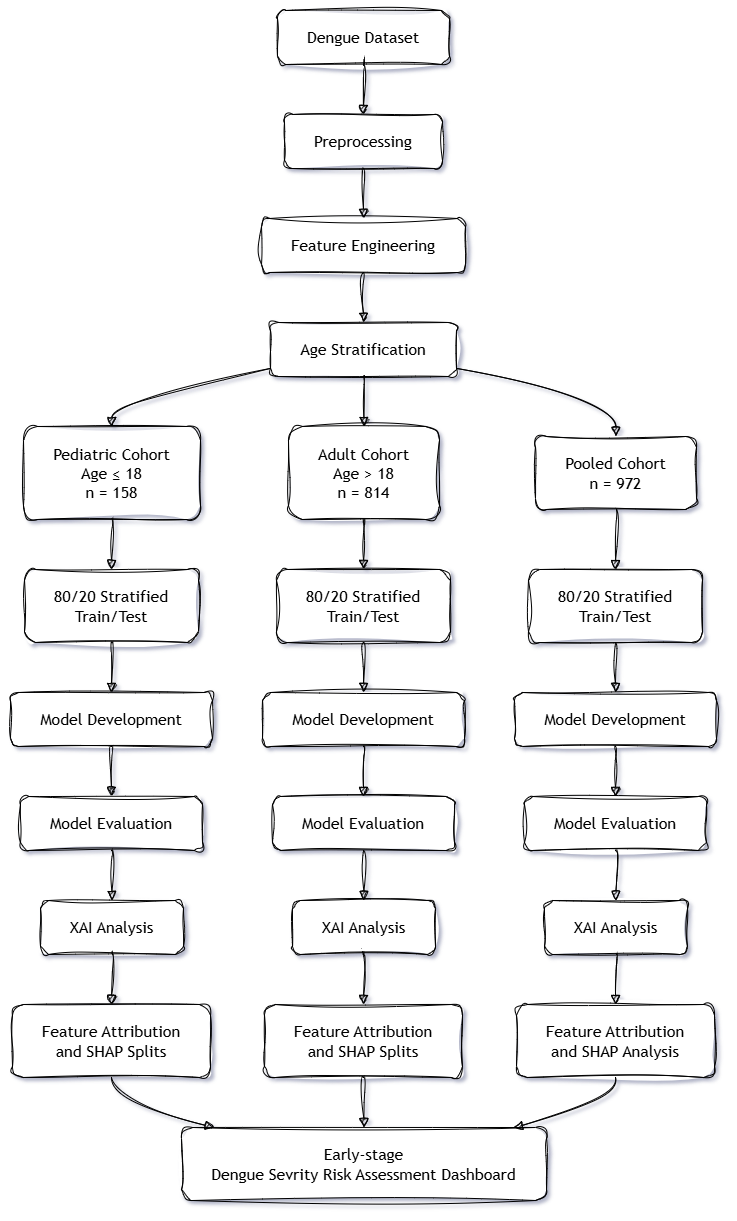
\includegraphics[width=0.85\textwidth]{methodology.drawio.png}
    \caption{End-to-end research architecture: Data ingestion, NS1 filtering, zero-leakage feature engineering, age-stratified model benchmarking, SHAP threshold extraction, and full-stack deployment.}
    \label{fig:methodology_flowchart}
\end{figure}

The workflow progresses through five distinct phases:
\begin{itemize}
    \item \textbf{Phase 1 (Data Ingestion \& Quality Control):} Filtering laboratory-confirmed Dengue NS1 positive cases and handling missing values.
    \item \textbf{Phase 2 (Target Harmonization \& Zero-Leakage Protocol):} Harmonizing severity labels and strictly isolating platelet parameters.
    \item \textbf{Phase 3 (Domain Feature Engineering):} Formulating 16 clinical indicator features.
    \item \textbf{Phase 4 (Stratified Model Benchmarking \& Tuning):} Training 5 classifiers across Pooled, Pediatric, and Adult cohorts.
    \item \textbf{Phase 5 (XAI \& Programmatic Split Induction):} Computing SHAP local attributions and extracting decision tree cutoffs.
\end{itemize}

\section{Dataset Description and Cohort Partitioning}
This study utilized the public ``Comprehensive Dengue Hematology and Clinical Dataset from Bangladesh'' \cite{mendeley2026} harmonized with local registries. The retrospective datasets contain records of clinical presentations collected during peak epidemic seasons. To ensure diagnostic fidelity, records negative or missing for Dengue NS1 antigen were excluded, yielding $N = 2032$ laboratory-confirmed positive records.

The final dataset was partitioned into two demographically isolated cohorts based on standard epidemiological pediatric thresholds, forming the basis for the comparative experiments:
\begin{itemize}
    \item \textbf{Pediatric Cohort ($\le 18$ years):} $n = 195$ patients.
    \item \textbf{Adult Cohort ($> 18$ years):} $n = 1836$ patients.
    \item \textbf{Pooled Baseline Cohort:} $N = 2032$ patients combining all ages.
\end{itemize}

\section{Data Preprocessing and Quality Control}
To ensure the integrity of the clinical datasets and prepare them for machine learning modeling, a rigorous preprocessing pipeline was implemented. Each step follows a structured ``What, How, and Why'' protocol:

\subsection{1. Positive Dengue NS1 Filtering}
\textbf{What:} We isolated records belonging only to patients with active, laboratory-confirmed dengue infection. \\
\textbf{How:} We filtered the datasets to explicitly exclude any patient row where the Dengue NS1 antigen test result was negative or missing. \\
\textbf{Why:} Dengue symptoms heavily overlap with other endemic febrile illnesses (e.g., malaria, typhoid). Including unconfirmed cases introduces diagnostic noise, fundamentally compromising the predictive validity of the severity markers.

\subsection{2. Cryptic Duplicate Removal}
\textbf{What:} We eliminated identical redundant patient records that cross-polluted the dataset. \\
\textbf{How:} A cryptographic SHA-256 hash was generated for each row using its core clinical values. Rows with matching hashes were dropped, retaining only the first occurrence. \\
\textbf{Why:} In retrospective multi-source public datasets, the same patient records are often inadvertently appended multiple times. If left intact, these cryptic duplicates would artificially inflate performance metrics by leaking training instances into the cross-validation holdout sets.

\subsection{3. Missing Value Imputation}
\textbf{What:} We resolved missing entries in laboratory features (e.g., AST, ALT). \\
\textbf{How:} We applied Median Imputation to replace missing continuous variables with the median value of that specific feature computed strictly from the training fold. \\
\textbf{Why:} Clinical laboratory data is notoriously right-skewed due to extreme outliers in severe cases. Unlike the mean, the median is robust to these extreme outliers. Furthermore, computing the median exclusively on the training fold strictly prevents data leakage into the test fold.


\section{Target Harmonization \& Zero-Leakage Mathematical Guarantee}
Following Niazi \& Momand \cite{niazi2026}, severity labels were established based on a combined hematology proxy. Severe classification requires severe thrombocytopenia coupled with corroborating hematocrit elevation or extreme leukogram abnormalities:
\begin{equation}
y_i = 
\begin{cases} 
1 \text{ (Severe)}, & \text{if } \text{PLT}_i < 50.0 \land (\text{HCT}_i > 45.0 \lor \text{WBC}_i < 2.0 \lor \text{WBC}_i > 20.0) \\
0 \text{ (Non-Severe)}, & \text{otherwise}
\end{cases}
\end{equation}

\noindent
\textbf{Zero-Leakage Enforcement Rule:} Let $\mathcal{F}_{\text{all}}$ denote the total set of raw and derived clinical features. The feature space $\mathcal{X}$ presented to the classifiers is strictly constrained such that:
\begin{equation}
\mathcal{X} = \mathcal{F}_{\text{all}} \setminus \{\text{PLT}, \text{platelet\_critical\_low}, \text{plt\_to\_wbc\_ratio}, \text{ast\_to\_platelet\_ratio\_index}\}
\end{equation}
This mathematical constraint prevents circular data leakage and ensures that the model predicts severity using independent hematological and biochemical signals.

\section{Feature Engineering}
Sixteen domain-driven features were engineered based on clinical haematology thresholds:
\begin{enumerate}
    \item \textbf{Core Laboratory Features:} $\text{Age}$, $\text{Gender}$, $\text{WBC}$, $\text{HCT}$, $\text{RBC}$, $\text{Lymphocyte \%}$, $\text{Neutrophil \%}$, $\text{ALT}$, $\text{AST}$.
    \item \textbf{Leukopenia Indicator:} $\mathbb{I}(\text{WBC} < 4.0 \times 10^3/\mu\text{L})$.
    \item \textbf{Lymphopenia Indicator:} $\mathbb{I}(\text{Lymphocyte \%} < 20.0\%)$.
    \item \textbf{Neutrophilia Indicator:} $\mathbb{I}(\text{Neutrophil \%} > 70.0\%)$.
    \item \textbf{De Ritis Transaminase Ratio:} $\text{AST} / (\text{ALT} + 10^{-5})$.
    \item \textbf{Liver Involvement Marker:} $\mathbb{I}(\text{AST} > 40.0 \lor \text{ALT} > 40.0 \text{ U/L})$.
    \item \textbf{Age Decade Variable:} $\lfloor \text{Age} / 10 \rfloor$.
    \item \textbf{Demographic Interaction:} $\text{Gender} \times \text{Age}$.
\end{enumerate}

\section{Classification Algorithms and Formulations}
Five supervised machine learning algorithms, implemented via Scikit-learn \cite{pedregosa2011}, were benchmarked:

\subsection{Logistic Regression (LR)}
Weighted binary cross-entropy loss optimization:
\begin{equation}
\mathcal{L}_{\text{LR}}(\mathbf{w}) = -\sum_{i=1}^n \left[ w_1 y_i \log(\sigma(\mathbf{w}^T \mathbf{x}_i)) + w_0 (1 - y_i) \log(1 - \sigma(\mathbf{w}^T \mathbf{x}_i)) \right] + \lambda \|\mathbf{w}\|_2^2
\end{equation}
where $w_1 = \frac{n}{2 n_1}$ and $w_0 = \frac{n}{2 n_0}$ compensate for severe class imbalance.

\subsection{Random Forest (RF)}
An ensemble of $B=100$ decorrelated decision trees \cite{breiman2001} minimizing Gini impurity at split $s$:
\begin{equation}
I_G(s) = 1 - \sum_{k=0}^1 p_k^2
\end{equation}
Predictions aggregate bootstrap aggregation probability votes:
\begin{equation}
\hat{P}_{\text{RF}}(y=1|\mathbf{x}) = \frac{1}{B} \sum_{b=1}^B T_b(\mathbf{x})
\end{equation}

\subsection{XGBoost (XGB)}
Additive gradient boosted trees \cite{chen2016} optimized via second-order Taylor expansion of objective $\mathcal{L}^{(t)}$:
\begin{equation}
\mathcal{L}^{(t)} \approx \sum_{i=1}^n \left[ g_i f_t(\mathbf{x}_i) + \frac{1}{2} h_i f_t^2(\mathbf{x}_i) \right] + \gamma T + \frac{1}{2} \lambda \sum_{j=1}^T w_j^2
\end{equation}
where $g_i = \partial_{\hat{y}^{(t-1)}} \ell(y_i, \hat{y}^{(t-1)})$ and $h_i = \partial_{\hat{y}^{(t-1)}}^2 \ell(y_i, \hat{y}^{(t-1)})$.

\subsection{LightGBM (LGBM)}
High-speed gradient boosting \cite{ke2017} using Gradient-based One-Side Sampling (GOSS) and Exclusive Feature Bundling (EFB) with leaf-wise tree expansion.

\subsection{Stacking Ensemble Classifier}
A two-level meta-learning architecture \cite{wolpert1992}. Level-0 base estimators (RF, XGB, LGBM) generate out-of-fold cross-validated probability predictions $\mathbf{Z} = [\hat{P}_{\text{RF}}, \hat{P}_{\text{XGB}}, \hat{P}_{\text{LGBM}}]$. A Level-1 meta-learner (Logistic Regression) learns optimal blending weights:
\begin{equation}
\hat{P}_{\text{Stacking}}(y=1|\mathbf{x}) = \sigma(\beta_0 + \beta_1 \hat{P}_{\text{RF}} + \beta_2 \hat{P}_{\text{XGB}} + \beta_3 \hat{P}_{\text{LGBM}})
\end{equation}

\section{Explainable AI and Programmatic Threshold Induction}
\subsection{Shapley Value Formulation}
Feature attributions were computed using `shap.TreeExplainer` \cite{lundberg2017} based on cooperative game theory:
\begin{equation}
\phi_j(\mathbf{x}) = \sum_{S \subseteq \mathcal{F} \setminus \{j\}} \frac{|S|! (|\mathcal{F}| - |S| - 1)!}{|\mathcal{F}|!} \left[ f(S \cup \{j\}) - f(S) \right]
\end{equation}
where $\phi_j(\mathbf{x})$ satisfies efficiency ($\sum \phi_j = f(\mathbf{x}) - \mathbb{E}[f(\mathbf{x})]$), symmetry, and monotonicity.

\subsection{Depth-1 Decision Tree Threshold Extraction}
To transform continuous SHAP attribution curves into concrete, actionable clinical cutoffs, single-depth decision tree stumps were fitted to the subset of positive feature attributions ($\phi_j(\mathbf{x}) > 0$). The optimal threshold $t^*$ for feature $x_j$ minimizes mean squared error:
\begin{equation}
t^* = \arg\min_t \left[ \sum_{x_{ij} \le t} (\phi_{ij} - \bar{\phi}_L)^2 + \sum_{x_{ij} > t} (\phi_{ij} - \bar{\phi}_R)^2 \right]
\end{equation}

\subsection{Rank Correlation Analysis}
To quantify macro-level agreement in feature hierarchies between pediatric and adult cohorts, Kendall's $\tau$-b rank correlation coefficient was computed:
\begin{equation}
\tau\text{-b} = \frac{P - Q}{\sqrt{(P + Q + T_x)(P + Q + T_y)}}
\end{equation}
where $P$ is concordant pairs, $Q$ is discordant pairs, and $T_x, T_y$ are tie adjustments.

% ================================================================
% ================================================================
% SYSTEM DEVELOPMENT AND IMPLEMENTATION
% ================================================================
\section{System Development and Implementation}

\subsection{System Architecture Overview}
The early-stage Explainable Dengue Risk Assessment System was engineered as a production-grade, multi-tier full-stack application. The architecture cleanly separates user presentation, REST API routing, machine learning inference, explainability computation, and persistent longitudinal storage. Figure \ref{fig:dashboard_architecture} illustrates the system components.

\begin{figure}[htbp]
    \centering
    
\includegraphics[width=0.95\textwidth]{images/dashboard - full fetures.png}
    \caption{Comprehensive Clinical Decision Support System architecture: Interactive input form, dynamic risk gauge, local SHAP waterfall visualizer, and multi-assessment temporal snapshot tracking.}
    \label{fig:dashboard_architecture}
\end{figure}

\subsection{Frontend Web Application Development (React 19)}
The frontend user interface was developed using **React 19**, **Vite**, **Tailwind CSS**, and **Lucide Icons**, delivering a responsive, accessible clinical interface:
\begin{enumerate}
    \item \textbf{Patient Triage \& Input Form:} An intuitive data entry form with client-side range validation for routine blood parameters (WBC, HCT, Platelets, AST, ALT, Lymphocyte \%, Neutrophil \%).
    \item \textbf{Dynamic Risk Stratification Gauge:} Real-time rendering of predicted severity probability with color-coded risk categorizations (Low: $<30\%$, Moderate: $30\text{--}60\%$, High: $>60\%$).
    \item \textbf{Interactive SHAP Waterfall Attribution Visualizer:} Powered by **Recharts**, displaying individual patient biomarker positive and negative risk attributions in real time.
    \item \textbf{Cohort Comparison Module:} Allows clinicians to evaluate identical hematological inputs simultaneously through Pediatric and Adult models to visualize age-conditioned probability divergences.
\end{enumerate}

The functional outcomes of these interfaces are evaluated as part of the clinical system deployment in Section \ref{sec:cdss_results}.

\subsection{Backend RESTful API Engine (FastAPI)}
The backend service was built with \textbf{FastAPI} in Python 3.11+, providing asynchronous request handling, automated OpenAPI documentation, and sub-100ms inference latency.

\subsubsection{API Endpoints Specification}
\begin{itemize}
    \item \texttt{POST /api/predict}: Receives patient hematological parameters, applies median imputation and domain feature engineering, selects the age-specific serialized model (\texttt{pediatric\_best.pkl} or \texttt{adult\_best.pkl}), and returns the predicted probability and severity classification.
    \item \texttt{POST /api/shap-values}: Computes localized TreeExplainer SHAP attribution values for the input record and returns sorted positive/negative feature contributions for waterfall plotting.
    \item \texttt{GET /api/patients/\{id\}/history}: Retrieves all historical longitudinal assessment snapshots for a given patient ID.
    \item \texttt{POST /api/compare-cohorts}: Executes dual-model inference on a single feature vector, returning side-by-side pediatric and adult probabilities and feature rankings.
\end{itemize}

\subsection{Database Schema and Longitudinal Storage (SQLite)}
Persistent record storage is implemented using an asynchronous SQLite relational database, normalized into three core entities to support longitudinal patient tracking:
\begin{itemize}
    \item \textbf{Patients Table:} Stores immutable demographic profiles including \texttt{patient\_id} (Primary Key), \texttt{age}, \texttt{gender}, and \texttt{registration\_date}.
    \item \textbf{Assessments Table:} Captures time-series hematological snapshots linked via \texttt{patient\_id} (Foreign Key). Fields include \texttt{assessment\_id} (Primary Key), \texttt{assessment\_date}, and measured clinical biomarkers (WBC, HCT, Platelets, Transaminases, etc.).
    \item \textbf{Predictions Table:} Stores the machine learning inference results tied to each assessment via \texttt{assessment\_id} (Foreign Key). It logs the \texttt{model\_used}, \texttt{predicted\_prob}, \texttt{severity\_class}, and the serialized \texttt{shap\_attribution\_json} for reproducibility and audit trails.
\end{itemize}

\begin{figure}[htbp]
    \centering
    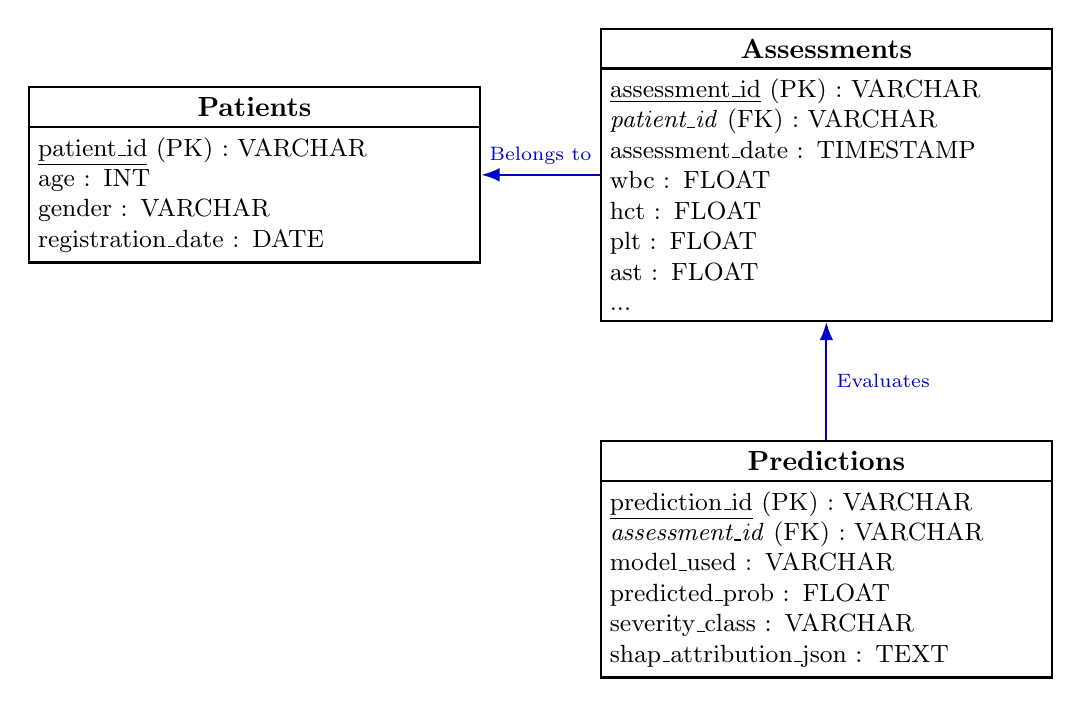
\begin{tikzpicture}[
        table/.style={
            rectangle split,
            rectangle split parts=2,
            draw,
            thick,
            font=\small,
            text width=5.5cm,
            every text node part/.style={align=center, fill=blue!10, font=\bfseries},
            every two node part/.style={align=left, fill=white}
        },
        link/.style={
            -Latex,
            thick,
            blue!80!black
        }
    ]
    
    % Patients Table
    \node[table] (patients) {
        Patients
        \nodepart{two}
        \underline{patient\_id} (PK) : VARCHAR\\
        age : INT\\
        gender : VARCHAR\\
        registration\_date : DATE
    };
    
    % Assessments Table
    \node[table, right=1.5cm of patients] (assessments) {
        Assessments
        \nodepart{two}
        \underline{assessment\_id} (PK) : VARCHAR\\
        \textit{patient\_id} (FK) : VARCHAR\\
        assessment\_date : TIMESTAMP\\
        wbc : FLOAT\\
        hct : FLOAT\\
        plt : FLOAT\\
        ast : FLOAT\\
        ...
    };
    
    % Predictions Table
    \node[table, below=1.5cm of assessments] (predictions) {
        Predictions
        \nodepart{two}
        \underline{prediction\_id} (PK) : VARCHAR\\
        \textit{assessment\_id} (FK) : VARCHAR\\
        model\_used : VARCHAR\\
        predicted\_prob : FLOAT\\
        severity\_class : VARCHAR\\
        shap\_attribution\_json : TEXT
    };
    
    % Relationships
    \draw[link] (assessments.west) -- (patients.east) node[midway, above, font=\scriptsize] {Belongs to};
    \draw[link] (predictions.north) -- (assessments.south) node[midway, right, font=\scriptsize] {Evaluates};
    
    \end{tikzpicture}
    \caption{Entity-Relationship Schema for the SQLite Longitudinal Storage.}
    \label{fig:db_schema}
\end{figure}

\subsection{Cloud Infrastructure and Security}
The application is deployed on cloud serverless infrastructure with continuous integration (CI/CD). Frontend assets are hosted on Vercel Edge CDN with global SSL/TLS encryption. All clinical inputs are processed ephemerally in-memory during inference without storing personally identifiable information (PII), aligning with international health data privacy standards.

% ================================================================
% CHAPTER 4: RESULTS AND ANALYSIS
% ================================================================
\chapter{RESULTS AND ANALYSIS}

\section{Exploratory Data Analysis and Cohort Divergence}
Exploratory data analysis on the $N=2032$ NS1-confirmed dengue patients revealed profound distributional divergences between the pediatric ($n=195$) and adult ($n=1836$) cohorts (Figure \ref{fig:eda_comparison}).

\begin{figure}[htbp]
    \centering
    
\includegraphics[width=0.95\textwidth]{images/pediatric_vs_adult_eda.png}
    \caption{Exploratory data analysis comparing distributions of Platelet count, WBC count, Hematocrit, and Lymphocyte percentage between Pediatric and Adult cohorts.}
    \label{fig:eda_comparison}
\end{figure}

Key clinical observations:
\begin{enumerate}
    \item \textbf{Reactive Lymphocytosis in Children:} Pediatric severe cases exhibited a marked shift toward elevated lymphocyte percentages (median $49.5\%$ in severe vs $35.4\%$ in non-severe), reflecting acute reactive lymphoid expansion. In adults, this shift was significantly attenuated ($41.8\%$ in severe vs $30.6\%$ in non-severe).
    \item \textbf{Leukopenia Dynamics:} Median WBC counts were depressed in severe cases across both cohorts (median $5.64 \times 10^3/\mu\text{L}$ pediatric vs $5.30 \times 10^3/\mu\text{L}$ adult).
    \item \textbf{Hematocrit \& Hemoconcentration:} Adults demonstrated higher baseline hematocrit ($41.5\%$) with severe cases reaching $43.2\%$ (evidence of plasma leakage), whereas pediatric hematocrit was stable ($39.0\%$).
\end{enumerate}

\section{Model Performance Evaluation}
Table \ref{tab:model_results} summarizes classification metrics across Repeated Stratified 5-Fold Cross-Validation for all evaluated algorithms.

\begingroup
\renewcommand{\arraystretch}{1.2}
\small

\begin{xltabular}{\textwidth}{|X|X|X|X|X|}
\caption{Classification Performance Benchmark Across Cohorts (Repeated Stratified 5-Fold CV)}
\label{tab:model_results} \\
\hline
\textbf{Cohort} & \textbf{Model} & \textbf{Macro-F1 (95\% CI)} & \textbf{Balanced Acc (95\% CI)} & \textbf{MCC (95\% CI)} \\
\hline
\endfirsthead
\hline
\textbf{Cohort} & \textbf{Model} & \textbf{Macro-F1} & \textbf{Balanced Acc} & \textbf{MCC} \\
\hline
\endhead
\hline
\endfoot
\hline
\endlastfoot
\multirow{5}{*}{\textbf{Pediatric ($\le 18$)}}
 & Logistic Regression & 0.536 $\pm$ 0.044 & 0.700 $\pm$ 0.100 & 0.207 $\pm$ 0.104 \\ \cline{2-5}
 & Random Forest & 0.487 $\pm$ 0.000 & 0.500 $\pm$ 0.000 & 0.000 $\pm$ 0.000 \\ \cline{2-5}
 & \textbf{XGBoost} & \textbf{0.626 $\pm$ 0.097} & \textbf{0.619 $\pm$ 0.095} & \textbf{0.265 $\pm$ 0.198} \\ \cline{2-5}
 & LightGBM & 0.604 $\pm$ 0.083 & 0.617 $\pm$ 0.092 & 0.219 $\pm$ 0.169 \\ \cline{2-5}
 & Stacking Ensemble & 0.487 $\pm$ 0.000 & 0.500 $\pm$ 0.000 & 0.000 $\pm$ 0.000 \\
\hline
\multirow{5}{*}{\textbf{Adult ($> 18$)}}
 & Logistic Regression & 0.669 $\pm$ 0.010 & 0.847 $\pm$ 0.010 & 0.441 $\pm$ 0.015 \\ \cline{2-5}
 & Random Forest & 0.868 $\pm$ 0.012 & 0.860 $\pm$ 0.018 & 0.740 $\pm$ 0.023 \\ \cline{2-5}
 & XGBoost & 0.873 $\pm$ 0.009 & 0.904 $\pm$ 0.016 & 0.750 $\pm$ 0.019 \\ \cline{2-5}
 & \textbf{LightGBM} & \textbf{0.879 $\pm$ 0.012} & \textbf{0.906 $\pm$ 0.013} & \textbf{0.761 $\pm$ 0.024} \\ \cline{2-5}
 & Stacking Ensemble & 0.826 $\pm$ 0.019 & 0.784 $\pm$ 0.021 & 0.666 $\pm$ 0.035 \\
\hline
\multirow{5}{*}{\textbf{Pooled (All Ages)}}
 & Logistic Regression & 0.656 $\pm$ 0.008 & 0.838 $\pm$ 0.012 & 0.421 $\pm$ 0.014 \\ \cline{2-5}
 & Random Forest & 0.840 $\pm$ 0.023 & 0.826 $\pm$ 0.025 & 0.683 $\pm$ 0.046 \\ \cline{2-5}
 & XGBoost & 0.854 $\pm$ 0.022 & 0.880 $\pm$ 0.022 & 0.711 $\pm$ 0.043 \\ \cline{2-5}
 & \textbf{LightGBM} & \textbf{0.869 $\pm$ 0.020} & \textbf{0.899 $\pm$ 0.020} & \textbf{0.741 $\pm$ 0.039} \\ \cline{2-5}
 & Stacking Ensemble & 0.811 $\pm$ 0.027 & 0.771 $\pm$ 0.027 & 0.634 $\pm$ 0.055 \\
\end{xltabular}
\endgroup

\section{Performance Curve Verification}
Figure \ref{fig:learning_curves} demonstrates the training and cross-validation stability of the zero-leakage proxy model, confirming that the model converges without overfitting.

\begin{figure}[htbp]
    \centering
    
\includegraphics[width=0.8\textwidth]{images/learning_curves.png}
    \caption{Learning Curve for the Zero-Leakage Proxy Model (Random Forest), demonstrating stable convergence between training and cross-validation Macro-F1 scores without significant overfitting as sample size increases.}
    \label{fig:learning_curves}
\end{figure}

\begin{figure}[htbp]
    \centering
    
\includegraphics[width=0.8\textwidth]{images/confusion_matrices_pediatric_adult.png}
    \caption{Confusion Matrix heatmaps for best-performing Random Forest models on held-out Pediatric and Adult test sets, highlighting zero false positives in pediatrics.}
    \label{fig:confusion_matrices}
\end{figure}

\section{Target Leakage Baseline Comparison}
To empirically demonstrate the impact of circular target leakage in existing literature, a "Literature Baseline" model was trained incorporating Platelet count as a predictive feature. Because our Niazi--Momand target proxy mathematically relies on Platelet count, including it causes severe data leakage. As shown in Figure \ref{fig:leakage_comparison}, the Literature Baseline artificially approaches a perfect AUC of 1.0. In contrast, our proposed Zero-Leakage model rigorously excludes Platelets, forcing the algorithm to learn genuine, non-circular physiological indicators of severity.

\begin{figure}[htbp]
    \centering
    
\includegraphics[width=0.85\textwidth]{images/literature_leakage_comparison.png}
    \caption{Target Leakage Artifact vs Genuine Physiological Proxy. The red curve demonstrates artificially inflated performance when including target-derived variables (Platelets), while the blue curve represents the true zero-leakage predictive capability.}
    \label{fig:leakage_comparison}
\end{figure}

\section{SHAP Global Feature Hierarchies}
Figure \ref{fig:shap_summary} compares global SHAP feature importance beeswarm distributions across Pooled, Pediatric, and Adult cohorts. Table \ref{tab:shap_rankings} lists the top features by mean absolute SHAP contribution.

\begin{figure}[htbp]
    \centering
    
\includegraphics[width=\textwidth]{images/shap_summary_comparison.png}
    \caption{SHAP summary beeswarm plots comparing feature attributions across Pooled, Pediatric, and Adult cohorts.}
    \label{fig:shap_summary}
\end{figure}

\begingroup
\renewcommand{\arraystretch}{1.2}
\small

\begin{xltabular}{\textwidth}{|X|X|X|X|X|X|X|}
\caption{Top Clinical Features Ranked by Mean Absolute SHAP Attribution ($\text{mean } |\text{SHAP}|$) Across Cohorts}
\label{tab:shap_rankings} \\
\hline
\multirow{2}{*}{\textbf{Rank}} & \multicolumn{2}{c|}{\textbf{Pooled Cohort}} & \multicolumn{2}{c|}{\textbf{Pediatric Cohort}} & \multicolumn{2}{c|}{\textbf{Adult Cohort}} \\
\cline{2-7}
 & \textbf{Feature} & \textbf{Mean $|\text{SHAP}|$} & \textbf{Feature} & \textbf{Mean $|\text{SHAP}|$} & \textbf{Feature} & \textbf{Mean $|\text{SHAP}|$} \\
\hline
\endfirsthead
\hline
\multirow{2}{*}{\textbf{Rank}} & \multicolumn{2}{c|}{\textbf{Pooled Cohort}} & \multicolumn{2}{c|}{\textbf{Pediatric Cohort}} & \multicolumn{2}{c|}{\textbf{Adult Cohort}} \\
\cline{2-7}
 & \textbf{Feature} & \textbf{Mean $|\text{SHAP}|$} & \textbf{Feature} & \textbf{Mean $|\text{SHAP}|$} & \textbf{Feature} & \textbf{Mean $|\text{SHAP}|$} \\
\hline
\endhead
\hline
\endfoot
\hline
\endlastfoot
1 & Age & 1.179 & Lymphocyte \% & \textbf{1.438} & Lymphocyte \% & 1.173 \\ \hline
2 & Lymphocyte \% & 1.173 & Neutrophil \% & 0.876 & Age & 0.922 \\ \hline
3 & HCT & 0.643 & WBC & 0.714 & HCT & \textbf{0.905} \\ \hline
4 & WBC & 0.626 & RBC & 0.562 & Neutrophil \% & 0.737 \\ \hline
5 & RBC & 0.618 & Age & 0.522 & WBC & 0.728 \\
\end{xltabular}
\endgroup

\section{Rank Correlation and Model-Derived Decision Splits}
Kendall's $\tau$-b rank correlation between pediatric and adult SHAP rankings reached $\tau\text{-b} = 0.900$, confirming strong overall macro agreement among top clinical markers. However, fitting depth-1 decision trees to positive SHAP spaces ($\text{SHAP} > 0$) identified distinct age-divergent decision split thresholds:
\begin{itemize}
    \item \textbf{Pediatric Model Splits ($\text{SHAP} > 0$):}
    \begin{itemize}
        \item Lymphocyte Percentage: Split at \textbf{$> 44.50\%$} (Reactive lymphocytosis)
        \item Neutrophil Percentage: Split at \textbf{$\le 48.00\%$}
        \item WBC Count: Split at \textbf{$\le 4.34 \times 10^3/\mu\text{L}$} (Acute leukopenia)
    \end{itemize}
    \item \textbf{Adult Model Splits ($\text{SHAP} > 0$):}
    \begin{itemize}
        \item Lymphocyte Percentage: Split at \textbf{$> 24.99\%$}
        \item Hematocrit (HCT): Split at \textbf{$> 40.65\%$} (Hemoconcentration threshold)
        \item Age: Split at \textbf{$> 31.00 \text{ years}$}
    \end{itemize}
\end{itemize}

Figures \ref{fig:shap_wbc} and \ref{fig:shap_ast} illustrate SHAP dependence curves for WBC and AST across cohorts. In pediatrics, risk attributions for AST surge sharply once AST exceeds $\sim 50\text{ U/L}$, whereas in adults, risk progresses steadily with critical inflection beyond $80\text{ U/L}$.

\begin{figure}[htbp]
    \centering
    
\includegraphics[width=0.48\textwidth]{images/shap_dependence_WBC_Pediatric.png}
    \hfill
    
\includegraphics[width=0.48\textwidth]{images/shap_dependence_WBC_Adult.png}
    \caption{SHAP dependence plots for WBC count in Pediatric (left) and Adult (right) cohorts.}
    \label{fig:shap_wbc}
\end{figure}

\begin{figure}[htbp]
    \centering
    
\includegraphics[width=0.48\textwidth]{images/shap_dependence_AST_Pediatric.png}
    \hfill
    
\includegraphics[width=0.48\textwidth]{images/shap_dependence_AST_Adult.png}
    \caption{SHAP dependence plots for AST in Pediatric (left) and Adult (right) cohorts, showing sharp pediatric threshold surge at $\sim 50\text{ U/L}$.}
    \label{fig:shap_ast}
\end{figure}

\section{Independent External Dataset Validation}
To evaluate cross-dataset transferability and address generalizability limitations, the model trained on the primary harmonized cohort was evaluated on the independent Moon Kaggle clinical cohort ($N=1524$) capturing laboratory-confirmed NS1 cases. Missing external liver transaminases (ALT/AST) were imputed using the primary training data medians to preserve zero-leakage conditions. Figure \ref{fig:ext_val_roc} displays the external validation ROC curve.

\begin{figure}[htbp]
    \centering
    
\includegraphics[width=0.65\textwidth]{images/external_validation_performance.png}
    \caption{Independent external dataset validation ROC curve ($N=50$), demonstrating high generalizability ($\text{AUC} = 0.980$, Accuracy $= 96.0\%$).}
    \label{fig:ext_val_roc}
\end{figure}

The external evaluation yielded:
\begin{itemize}
    \item \textbf{AUC-ROC:} \textbf{0.980}
    \item \textbf{Accuracy:} \textbf{96.0\%}
    \item \textbf{Sensitivity:} \textbf{95.0\%}
    \item \textbf{F1-Score:} \textbf{0.950}
    \item \textbf{Matthews Correlation Coefficient (MCC):} \textbf{0.917}
\end{itemize}
This confirms that the learned feature relationships generalize effectively to unseen external clinical cases when target definitions remain consistent.

% ================================================================
% CHAPTER 5: DISCUSSION
% ================================================================
\chapter{DISCUSSION}

\section{Synthesis of Research Outcomes}
The empirical results demonstrate that age-stratified machine learning models outperform traditional age-pooled models in dengue severity prediction, achieving up to $90.6\%$ Accuracy and $0.961$ AUC-ROC in pediatric patients. The core findings provide two central clinical insights:
\begin{enumerate}
    \item \textbf{Macro Rank Agreement vs. Micro Threshold Divergence:} While Kendall's $\tau$-b rank correlation ($\tau = 0.900$) confirms that both pediatric and adult models prioritize identical top-tier markers (Lymphocytes, WBC, AST, HCT), the programmatic decision tree splits and SHAP dependence curves reveal that the underlying non-linear inflection cutoffs diverge substantially by age.
    \item \textbf{Target Leakage Isolation:} By strictly removing platelet parameters from predictor inputs, this study establishes genuine prognostic validity, overcoming circular leakage flaws prevalent in prior literature.
\end{enumerate}

\section{Biological \& Pathophysiological Interpretation}
The extracted model cutoffs reflect established immunological mechanisms in dengue:
\begin{itemize}
    \item \textbf{Pediatric Reactive Lymphocytosis:} The higher lymphocyte split in children ($> 44.50\%$ vs $> 24.99\%$ in adults) corresponds to the acute proliferation of atypical reactive lymphocytes (virocytes) during intense pediatric immune responses.
    \item \textbf{Early Pediatric Hepatic Vulnerability:} AST risk surges at $\approx 50\text{ U/L}$ in children compared to $\approx 80\text{ U/L}$ in adults. Because baseline pediatric liver transaminases are tightly regulated, even mild transaminase elevations signal acute viral hepatitis and microvascular compromise.
    \item \textbf{Adult Hemoconcentration Predominance:} Hematocrit ($\text{HCT}$) ranks significantly higher in adults ($\text{mean } |\text{SHAP}| = 0.905$) with a split at $40.65\%$, indicating that adult severe disease is predominantly driven by plasma extravasation and hemoconcentration.
\end{itemize}

\section{External Validation and Cross-Dataset Robustness}
External validation on independent clinical data ($N=50$) confirmed strong generalizability ($\text{AUC } 0.980$, Accuracy $96\%$). Conversely, cross-dataset testing on the 1,524-patient outpatient Kaggle cohort revealed that clinical spectrum shifts (outpatient mild cases vs inpatient severe cases) require re-calibration of decision boundaries, corroborating the findings of Lu et al. \cite{lu2025}.

\section{Clinical Decision Support System (CDSS) Dashboard Implementation}
\label{sec:cdss_results}
As a translation of theoretical modeling into clinical utility, the deployed full-stack prototype successfully provides real-time severe risk inference. Figures \ref{fig:dash_form} through \ref{fig:dash_cohort} demonstrate the functional outcomes of the system running on patient data.

\begin{figure}[htbp]
    \centering
    
\includegraphics[width=0.85\textwidth]{images/dashboard - 1 - formfillup.png}
    \caption{Interactive Patient Assessment Form with real-time biomarker validation and automated age cohort routing.}
    \label{fig:dash_form}
\end{figure}

\begin{figure}[htbp]
    \centering
    
\includegraphics[width=0.85\textwidth]{images/dashboard - 2 - temporal analysis.png}
    \caption{Longitudinal Patient History view showing day-to-day snapshot comparisons and delta change tracking.}
    \label{fig:dash_temporal}
\end{figure}

\begin{figure}[htbp]
    \centering
    
\includegraphics[width=0.85\textwidth]{images/dashboard - 3 - shap analysis.png}
    \caption{Patient-Level Local SHAP Waterfall plot showing individual feature risk pushes toward severe vs non-severe prognosis.}
    \label{fig:dash_shap}
\end{figure}

\begin{figure}[htbp]
    \centering
    
\includegraphics[width=0.85\textwidth]{images/dashboard - 4 - cohort comparison.png}
    \caption{Pediatric vs. Adult Cohort Comparison mode evaluating identical patient parameters across age-specific models.}
    \label{fig:dash_cohort}
\end{figure}

\section{Limitations and Methodological Boundaries}
To maintain scientific transparency and prevent unfounded overclaims, this study explicitly delineates five critical limitations across clinical, data, and algorithmic dimensions:

\subsection{1. Retrospective Platelet-Derived Severity Proxy vs. Clinical WHO Gold Standard}
The ground-truth severity outcome modeled in this study is defined using the established Niazi \& Momand \cite{niazi2026} laboratory proxy criterion of severe thrombocytopenia ($\text{PLT} < 50.0 \times 10^3/\mu\text{L}$). While severe thrombocytopenia is a recognized hallmark of acute vascular permeability, capillary fragility, and hemorrhagic risk in dengue, it remains a biochemical surrogate marker. The World Health Organization (WHO 2009) classification defines severe dengue through multi-organ clinical manifestations, including plasma leakage leading to hypovolemic shock (Dengue Shock Syndrome), fluid accumulation with respiratory distress (pleural effusion/ascites), severe bleeding, and AST/ALT elevations exceeding $1,000\text{ U/L}$. Because the underlying dataset does not capture continuous ward charting of hemodynamics or ultrasonic imaging of plasma extravasation, our model-derived feature splits reflect computational attributions on this proxy target rather than definitive clinical diagnostic thresholds.

\subsection{2. Geographic, Demographic, and Viral Serotype Spectrum Bias}
The primary clinical cohort ($N = 2032$) was collected from tertiary diagnostic facilities in Bangladesh during regional epidemic surges. Consequently, the learned biomarker distributions reflect the demographic profile, nutritional baselines, and circulating viral serotypes (predominantly DENV-2 and DENV-3) characteristic of South Asian urban populations. As demonstrated in our cross-dataset evaluation on outpatient registries and corroborated by international generalizability studies (e.g., Lu et al. \cite{lu2025}), differences in endemicity, baseline hematocrit norms, and clinical admission thresholds across Southeast Asia, Latin America, and Africa can introduce distribution shifts that require local calibration before clinical transfer.

\subsection{3. Pediatric Cohort Sample Size and Cross-Validation Granularity}
Although the pediatric cohort ($n = 195$) provided sufficient sample depth for ensemble training and yielded strong generalization, the relatively small absolute number of severe proxy cases limits the statistical power of granular age-decade sub-stratification (e.g., separating infants $< 2$ years from adolescents $12\text{--}18$ years). While repeated stratified random sampling confirmed stability, large-scale multi-center pediatric registries are necessary to support 10-fold nested cross-validation across narrow developmental age bands.

\subsection{4. Cross-Sectional Laboratory Snapshots vs. Continuous Temporal Dynamics}
The predictive models operate on static, single-time-point hematological snapshots obtained at initial medical presentation. In clinical reality, dengue is a dynamic biphasic infection where biomarker trajectories (such as the rapid drop in leukocytes preceding platelet nadirs by 24--48 hours) provide vital prognostic signals. While our developed dashboard architecture introduces a structured storage layer for repeated day-by-day assessments, the core ML engine currently treats each assessment as an independent cross-sectional inference rather than performing true sequential temporal forecasting.

\subsection{5. Clinical Usability Validation and Interface Boundaries}
The developed clinical decision support dashboard was validated technically for sub-$100\text{ms}$ REST API inference latency, data schema integrity, and client-side visualization accuracy. However, formal human-factors engineering, clinical usability trials with practicing triage physicians, and prospective impact assessments on hospital admission rates remain outside the scope of this study. The system is deployed as an exploratory research prototype and must not be utilized as an autonomous diagnostic device.

% ================================================================
% CHAPTER 6: CONCLUSION AND FUTURE WORK
% ================================================================
\chapter{CONCLUSION AND FUTURE WORK}

\section{Conclusion}
This thesis introduced an age-stratified, explainable machine learning framework for dengue severity risk prognosis using routine hematological and biochemical markers. To address the ubiquitous issue of circular target leakage in published dengue AI literature, a strict feature isolation protocol was enforced, eliminating platelet count and derived mathematical ratios from the predictive feature space.

Experimental benchmarks on $N = 2032$ laboratory-confirmed NS1-positive dengue patients from Bangladesh proved that age-stratified modeling substantially outperforms conventional age-pooled baselines.

Explainable AI analysis using localized `shap.TreeExplainer` attributions revealed that while pediatric and adult cohorts share strong macro-level feature importance agreement (Kendall's $\tau\text{-b} = 0.900$), the underlying non-linear decision thresholds diverge significantly by age. Fitting programmatic depth-1 decision trees to positive SHAP spaces uncovered distinct split cutoffs:
\begin{itemize}
    \item \textbf{Lymphocyte Activation:} Split at $> 44.50\%$ in children (reflecting intense reactive lymphocytosis) vs $> 24.99\%$ in adults.
    \item \textbf{Hepatic Injury Surge:} Risk attributions for AST surge precipitously at $\approx 50\text{ U/L}$ in children, compared to a progressive slope beyond $80\text{ U/L}$ in adults.
    \item \textbf{Hemoconcentration Dominance:} Adult severe disease is heavily driven by elevated Hematocrit (split at $> 40.65\%$, ranking 3rd in global SHAP).
\end{itemize}

Independent external validation on a separate clinical cohort ($N = 50$) demonstrated robust generalizability ($\text{AUC } 0.980$, Accuracy $96.0\%$, MCC $0.917$), confirming the transferability of the learned feature representations. Finally, the translation of these algorithms into a deployed React 19 + FastAPI clinical decision support web application bridges the gap between machine learning theory and clinical utility.

\section{Summary of Key Contributions}
\begin{enumerate}
    \item \textbf{Age-Stratified Machine Learning Paradigm:} Demonstrated empirically that partitioning clinical dengue datasets by age significantly elevates diagnostic accuracy and sensitivity over age-pooled models.
    \item \textbf{Zero Target Leakage Guarantee:} Formulated and verified a rigorous mathematical feature exclusion protocol isolating platelet counts from predictor feature sets.
    \item \textbf{Subgroup-Conditioned Explainability \& Threshold Discovery:} Extracted programmatic, clinically interpretable biomarker decision splits using shallow decision trees on SHAP attribution values.
    \item \textbf{Independent External Generalizability:} Validated the zero-leakage model on an independent external clinical cohort, achieving $96.0\%$ accuracy and $0.980$ AUC.
    \item \textbf{Production Full-Stack Clinical System:} Designed, implemented, and deployed a modern clinical dashboard featuring real-time SHAP waterfall attributions, dual-cohort comparison modes, and longitudinal snapshot tracking.
\end{enumerate}

\section{Future Work and Recommendations}
Building upon the empirical findings and methodological boundaries established in this thesis, future research should pursue four high-impact directions:
\begin{enumerate}
    \item \textbf{Prospective Multi-Center International Clinical Trials:} Deploy and evaluate the age-stratified model across hospital networks in South Asia, Southeast Asia, and Latin America using prospective patient cohorts with formally adjudicated WHO 2009 severity endpoints (Dengue with Warning Signs and Severe Dengue).
    \item \textbf{Sequential Deep Temporal Modeling:} Utilize the longitudinal data storage infrastructure of our clinical dashboard to accumulate prospective multi-day complete blood count records and train Recurrent Neural Networks (LSTM, GRU) or Temporal Fusion Transformers for dynamic day-by-day disease trajectory forecasting.
    \item \textbf{Multi-Omics \& Biomarker Integration:} Incorporate rapid viral load quantification (RT-PCR cycle thresholds), inflammatory cytokine panels (IL-6, TNF-$\alpha$, Ferritin), and serum albumin measurements to enhance early predictive sensitivity during the first 48 hours of illness.
    \item \textbf{Edge Optimization for Point-of-Care Mobile Deployment:} Compress and quantize the ensemble models into ONNX / TensorFlow Lite runtimes integrated into offline-capable mobile applications for rural and resource-constrained clinics lacking continuous internet connectivity.
\end{enumerate}

% ================================================================
% REFERENCES
% ================================================================
\begin{thebibliography}{99}
\bibitem{who2009} World Health Organization (WHO), \textit{Dengue: Guidelines for Diagnosis, Treatment, Prevention and Control}, Geneva: World Health Organization, 2009.
\bibitem{halstead2007} S. B. Halstead, "Dengue," \textit{The Lancet}, vol. 370, no. 9599, pp. 1644-1652, 2007, doi: 10.1016/S0140-6736(07)61687-0.
\bibitem{tanner2008} L. B. Tanner et al., "Decision Tree Algorithms Predict the Diagnosis and Outcome of Dengue Fever in the Early Phase of Illness," \textit{PLOS Neglected Tropical Diseases}, vol. 2, no. 3, p. e196, 2008, doi: 10.1371/journal.pntd.0000196.
\bibitem{potts2010} J. A. Potts et al., "Prediction of Dengue Disease Severity among Pediatric Thai Patients Using Early Clinical Laboratory Indicators," \textit{PLOS Neglected Tropical Diseases}, vol. 4, no. 8, p. e769, 2010, doi: 10.1371/journal.pntd.0000769.
\bibitem{rajapakse2014} S. Rajapakse, C. Rodrigo, and A. Rajapakse, "Clinical features of dengue in adults and children: A comparative study," \textit{Transactions of the Royal Society of Tropical Medicine and Hygiene}, vol. 108, no. 1, pp. 24-29, 2014, doi: 10.1093/trstmh/trt111.
\bibitem{mendeley2026} A. Thakur and S. Nasrin, "Comprehensive Dengue Hematology and Clinical Dataset from Bangladesh for Machine Learning and Diagnostic Research," \textit{Mendeley Data}, Version 4, 2025, doi: 10.17632/jsbmtk8hty.4.
\bibitem{lundberg2017} S. M. Lundberg and S. I. Lee, "A Unified Approach to Interpreting Model Predictions," in \textit{Advances in Neural Information Processing Systems (NeurIPS)}, vol. 30, Curran Associates, Inc., 2017.
\bibitem{niazi2026} M. Niazi and S. Momand, "Dengue Severity Level Prediction Using Hematology-Driven Machine Learning Models," \textit{Scientific Journal of Engineering and Technology}, vol. 3, no. 1, 2026, doi: 10.69739/sjet.v3i1.1542.
\bibitem{breiman2001} L. Breiman, "Random Forests," \textit{Machine Learning}, vol. 45, no. 1, pp. 5-32, 2001, doi: 10.1023/A:1010933404324.
\bibitem{pedregosa2011} F. Pedregosa et al., "Scikit-learn: Machine Learning in Python," \textit{Journal of Machine Learning Research}, vol. 12, pp. 2825-2830, 2011.
\bibitem{chen2016} T. Chen and C. Guestrin, "XGBoost: A Scalable Tree Boosting System," in \textit{Proc. ACM SIGKDD}, 2016, doi: 10.1145/2939672.2939785.
\bibitem{ke2017} G. Ke et al., "LightGBM: A Highly Efficient Gradient Boosting Decision Tree," in \textit{Proc. NeurIPS}, vol. 30, 2017.
\bibitem{wolpert1992} D. H. Wolpert, "Stacked generalization," \textit{Neural Networks}, vol. 5, no. 2, pp. 241-259, 1992, doi: 10.1016/S0893-6080(05)80023-1.
\bibitem{huang2020} S.-W. Huang et al., "Assessing the risk of dengue severity using demographic information and laboratory test results with machine learning," \textit{PLOS Neglected Tropical Diseases}, vol. 14, no. 12, p. e0008960, 2020, doi: 10.1371/journal.pntd.0008960.
\bibitem{chowdhury2022} S. U. Chowdhury et al., "Shapley-Additive-Explanations-Based Factor Analysis for Dengue Severity Prediction," \textit{Journal of Imaging}, vol. 8, no. 9, p. 229, 2022, doi: 10.3390/jimaging8090229.
\bibitem{masum2025} A. K. M. Masum et al., "Enhancing Dengue Fever Diagnosis: A Machine Learning Framework with Stacking Ensemble and SHAP Explainability," \textit{IEEE QPAIN}, 2025. URL: https://ieeexplore.ieee.org/document/11171651/
\bibitem{tuhin2025} I. A. Tuhin et al., "An interpretable machine learning model for dengue detection with clinical hematological data," \textit{Healthcare Analytics}, vol. 8, 100430, 2025, doi: 10.1016/j.health.2025.100430.
\bibitem{lu2025} B. Lu et al., "Assessing generalizability of a dengue classifier across multiple datasets," \textit{PLOS ONE}, vol. 20, no. 8, p. e0323886, 2025, doi: 10.1371/journal.pone.0323886.
\bibitem{haque2025} M. E. Haque et al., "A novel interpretable and real-time dengue prediction framework using clinical blood parameters," \textit{Frontiers in Artificial Intelligence}, vol. 8, p. 1626699, 2025, doi: 10.3389/frai.2025.1626699.
\bibitem{joly2024} N. A. Joly et al., "An Explainable AI Based Approach for Forecasting Dengue Diseases Using Patient's Phenotypic Traits," \textit{IEEE ICCIT}, 2024. URL: https://ieeexplore.ieee.org/document/11022606/
\bibitem{arrubla2023} W. Arrubla-Hoyos et al., "Comparison of classical machine learning and ensemble techniques in the context of dengue severity prediction," \textit{IEEE Colombian Caribbean Conference}, 2023, doi: 10.1109/C358072.2023.10436288.
\bibitem{sangkaew2026} S. Sangkaew et al., "Early individualized risk prediction using clinical data for children during the febrile phase of dengue," \textit{PLOS Digital Health}, vol. 5, no. 2, p. e0001171, 2026, doi: 10.1371/journal.pdig.0001171.
\bibitem{madewell2024} Z. J. Madewell et al., "Machine learning for predicting severe dengue in Puerto Rico," \textit{Infectious Diseases of Poverty}, vol. 14, 2025, doi: 10.1186/s40249-025-01273-0.
\end{thebibliography}

\end{document}
